\documentclass[hyperref={pdfpagelabels=false}]{beamer}
%\usepackage{href}
\usepackage{listings}
\usepackage[utf8]{inputenc}
\setbeamertemplate{section in toc}[sections numbered]
\setbeamertemplate{subsection in toc}[subsections numbered]
\newcommand{\pu}{PostgreSQL Überblick}
\newcommand{\rsql}{Rekursiver SQL Aufruf}
\newcommand{\tit}{Ausgewählte Systeme Postgres }
\newcommand{\parcht}{Postgres Architektur}
\newcommand{\mergebnisse}{Messergebnisse pgBench}
\newcommand{\storedproc}{Stored Procedure}
\newcommand{\pgbench}{pgBench}
\newcommand{\konzepte}{Konzepte für rekursive Anfragen}
\newcommand{\fazit}{Fazit}
\usepackage{pdfpages}
\usepackage{tikz}
\usepackage{fancybox}
\usepackage{geometry}
\usepackage{pdflscape}
\usepackage{pgfplots}
\usepackage{filecontents}
%\usepackage{pgfplots}
\usepackage{pgfplotstable}
%\geometry{bottom=0.9in}
\usepackage{fancyhdr}
\setbeamertemplate{footline}[text line]{
	\parbox{\linewidth}{\vspace*{-20pt} \hyperlink{tableofcontent}{
\includegraphics[scale=0.03]{../images/rhein-sieg.jpg}} \hspace{1cm} \tit \hfill\insertshortauthor\hfill\insertpagenumber}}
\setbeamertemplate{navigation symbols}{}
\author{Jennifer Wittling, Rolf Kimmelmann, Jan Löffelsender}
\title{\tit}
\usepackage{lmodern}
\usepackage{amsmath}
\usepackage{graphicx}
\setcounter{tocdepth}{1}

\pgfplotsset{
discard if/.style 2 args={
    x filter/.code={
    \edef\tempa{\thisrow{#1}}
    \edef\tempb{#2}
    \ifx\tempa\tempb
    \def\pgfmathresult{inf}
    \fi
    }
},
discard if not/.style 2 args={
x filter/.code={
\edef\tempa{\thisrow{#1}}
\edef\tempb{#2}
\ifx\tempa\tempb
\else
\def\pgfmathresult{inf}
\fi
}
}}


\begin{document}

\begin{filecontents}{data.csv}
{Occurences}, {keyword}
15, StoredProcedure
25, InnerJoin
88, selectWithUnionAll
124, SubSelectGeneriert
126, SubSelect
192, selectWithUnion
\end{filecontents}
\tikzstyle{node} = [text width=2em, text centered]
%\lstset{language=Python}
%\lstset{language=Python}

\begin{frame}
\titlepage
\end{frame} 

\begin{frame}
\frametitle{Agenda}
\hypertarget{tableofcontent}{}
\tableofcontents
\end{frame} 

\section{PostgreSQL Überblick}
%\label{anforderung} 
	\begin{frame}
		\frametitle{\pu}
		Postgres ist ein Datenbankmanagementsystem mit folgenden Eigenschaften :
		\begin{itemize}
			\item Objektrelational
			\item ACID konform
            \item CRUD konform
            \item Hersteller: PostgreSQL Global Development Group, ursprünglich University of California
            \item Zielgruppe: Telekommunikationsunternehmen für Ordermanagement System.
		\end{itemize}
	\end{frame}

\section{Postgres Architektur}
%\label{anforderung}
\begin{frame}
	\frametitle{\parcht}
	\centering
	\begin{figure}
		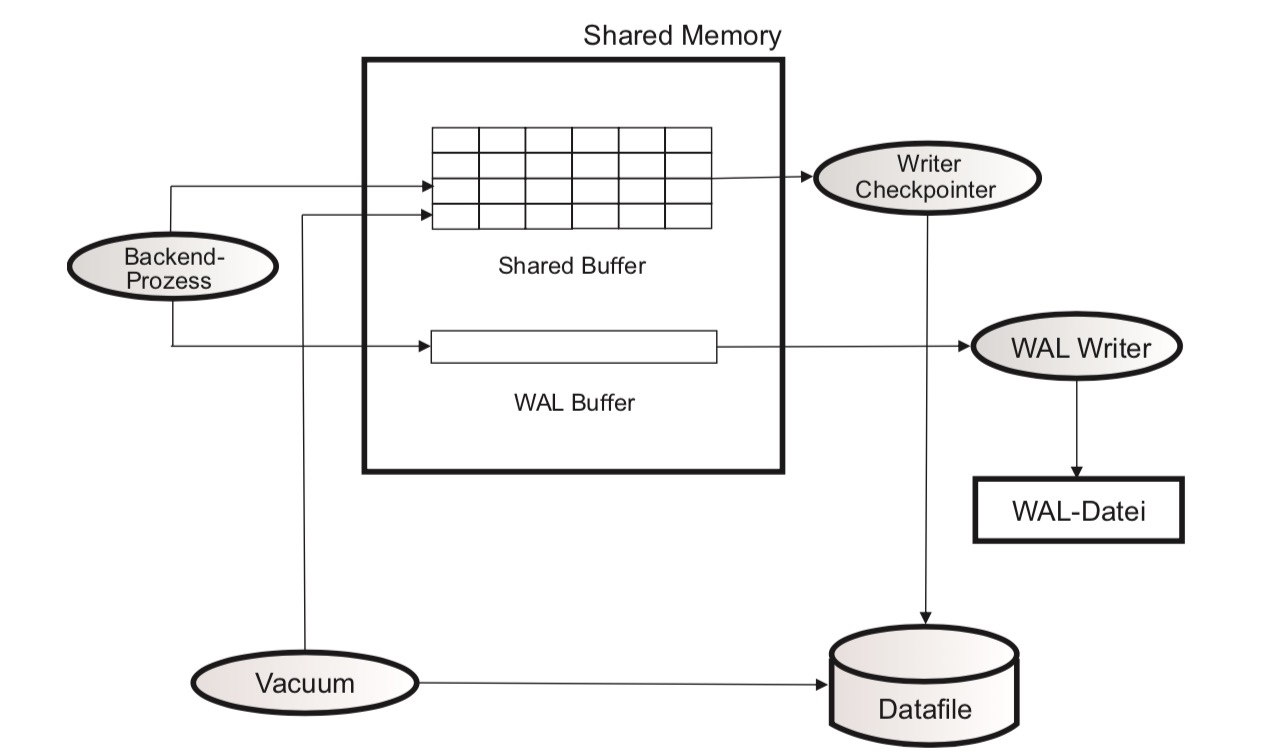
\includegraphics[scale=0.2]{../images/postgresArchitektur.jpg}
	\end{figure}
\end{frame}

\section{Konzepte für rekursive Anfragen}
\begin{frame}
    \frametitle{\konzepte}
        \center
            Nächste Seite

\end{frame}

    {
    \setbeamercolor{background canvas}{bg=}
    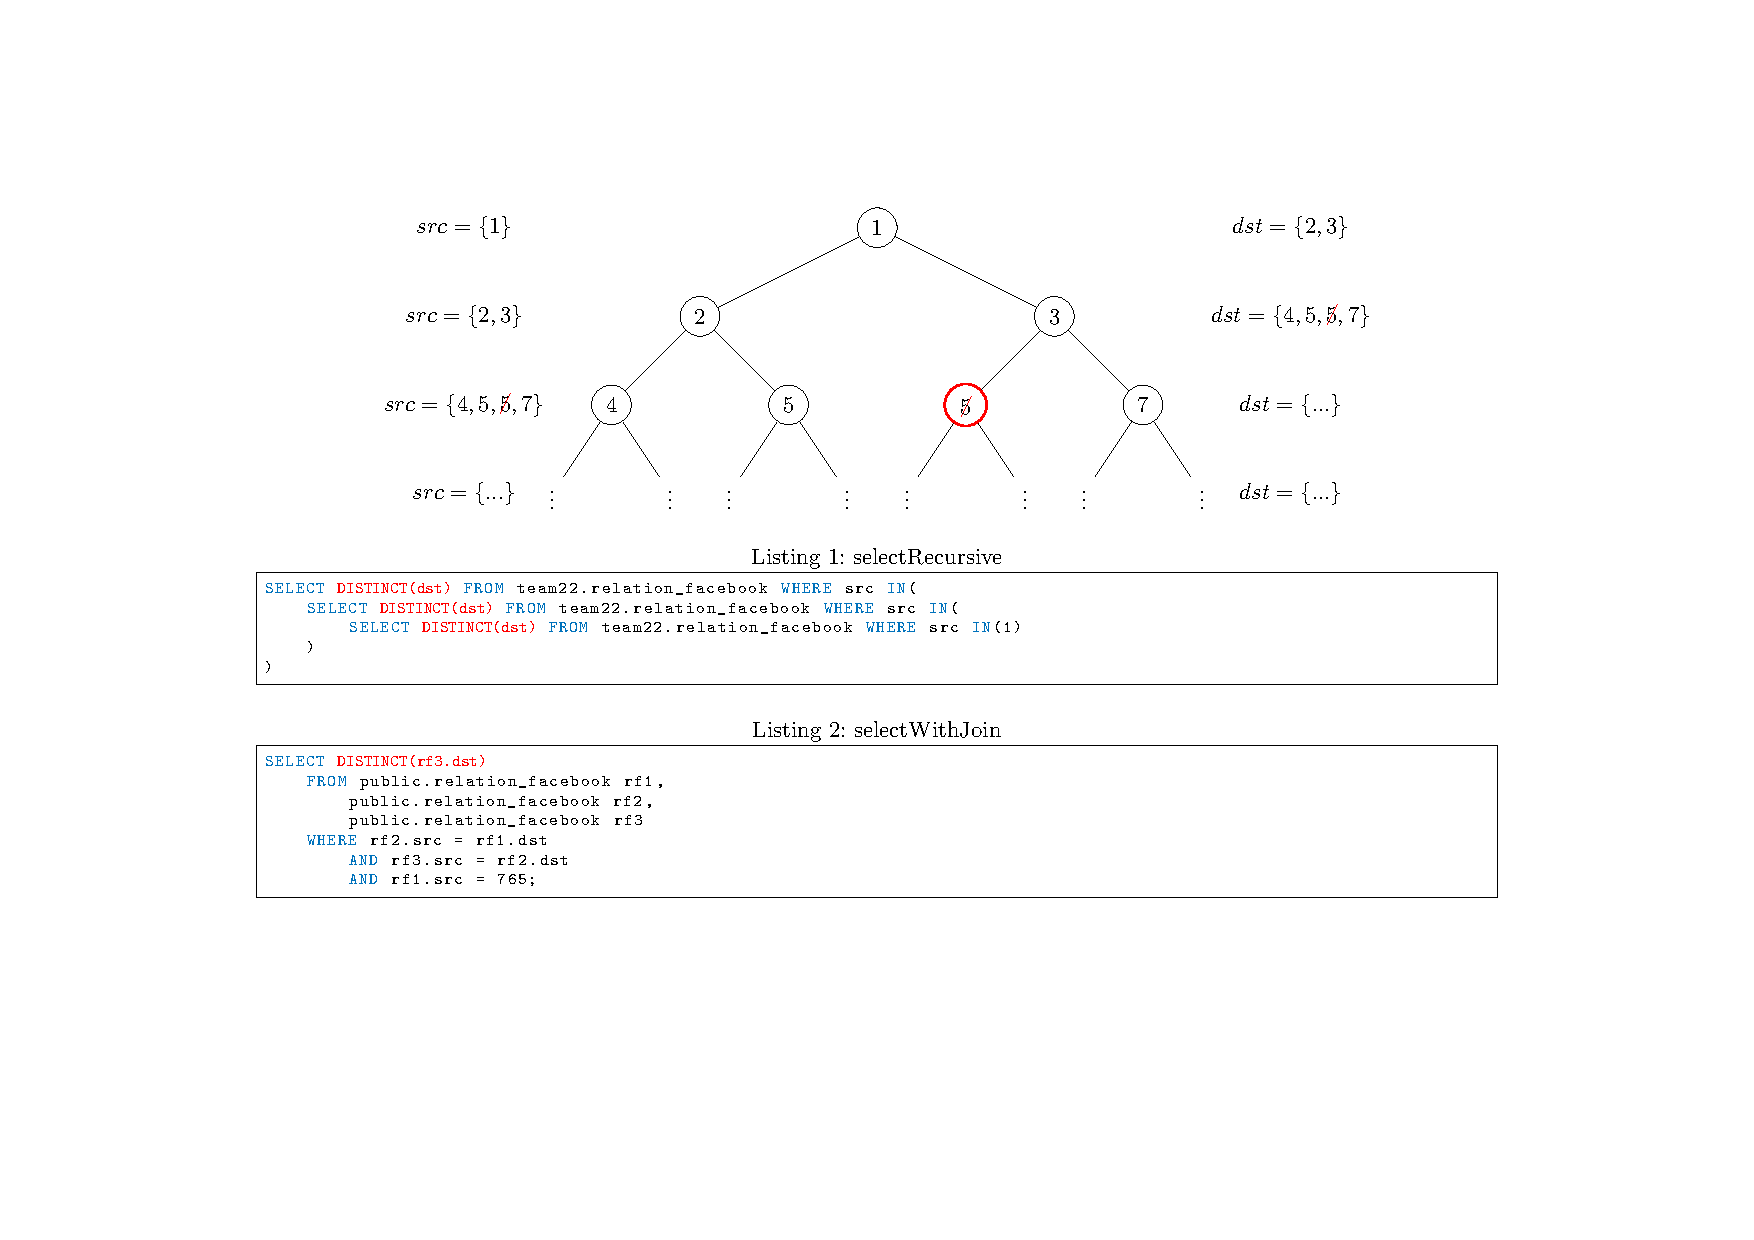
\includepdf[pages=-,fitpaper]{RecursiveSelect.pdf}
    }

%\section{StoredProcedure}
%%\label{anforderung}
%	\begin{frame}
%		\frametitle{\storedproc}
%
%	\end{frame}

\section{pgBench}
\begin{frame}
    \frametitle{\pgbench}
    \begin{itemize}
        \item Tool zur Durchführung von Benchmark-Tests
        \item Bei einem Benchmark-Test wird eine Menge von SQL-Statements beliebig oft wiederholt.
        \item pgBench berechnet die Anzahl der Transaktionen pro Sekunde
    \end{itemize}
\end{frame}
\section{Messergebnisse}
\begin{frame}
	\frametitle{\mergebnisse}
	\centering
	\begin{figure}
        \pgfplotstablegetrowsof{data.csv}
        \edef\numberofrows{\pgfplotsretval}
		\begin{tikzpicture}
            \begin{axis}[
            /pgf/number format/.cd,1000 sep={},
            width=0.8\linewidth,height=6cm,
            xbar,/pgf/bar shift=0pt,
            xmin=0, xmax=250,
            xtick=\empty,
            enlarge x limits={value=0.1, upper},
            enlarge y limits=0.1,
            ytick={0,...,\numberofrows},
            y dir=reverse,
            xlabel= {Transaktionen Pro Sekunde},
%            ylabel = {Verfahren},
            y tick label style={major tick length=0pt},
            yticklabels from table={data.csv}{[index]1},
            nodes near coords, nodes near coords align=horizontal
            ]

                \addplot [draw,fill=blue!50,discard if={keyword}{test}
                ] table [
                y expr=\coordindex,
                x index=0,col sep=comma
                ]{data.csv};

                \addplot [draw,fill=orange,discard if not={keyword}{test}] table [
                y expr=\coordindex,
                x index=0,col sep=comma
                ]{data.csv};
            \end{axis}
		\end{tikzpicture}
	\end{figure}
\end{frame}

\section{Fazit}
\begin{frame}
    \frametitle{\fazit}
    \begin{itemize}
        \item Rekursives Select per Standard SQL ist am schnellsten
        \item Rekursive Stored Procedures sind sehr langsam (kann aber auch an Implementierung liegen)
%        \item Reukrsives Traversieren mit Hilfe von StoredProcedures, InnerJoin und SubSelects nicht vergleichbar mit rekursiven Select per Standard SQL
    \end{itemize}
\end{frame}
\end{document}



